% !TEX root = main.tex

%%%%%%%%%%%%%%%%%%%%%%%%%%%%%%%%%%%%%%%%%%%%%%%%%%%%%%%%%%%%%%%%%%%%%%%%%%%%%%%%%%%%%%%%%%%%%%%%
\section{実験}
%%%%%%%%%%%%%%%%%%%%%%%%%%%%%%%%%%%%%%%%%%%%%%%%%%%%%%%%%%%%%%%%%%%%%%%%%%%%%%%%%%%%%%%%%%%%%%%%

\subsection{実験器具}
TEKTRONIX TBS1022 オシロスコープ,ソレノイドコイル,高電圧パルス大電流発生
電源,セメント抵抗$(1\Omega)$,可変抵抗$(<20\Omega)$

\newpage

\subsection{実験方法}
\subsubsection{セットアップ}
\begin{enumerate}
    \item 図1のように回路を作成する.
    \item 充電電圧調整ダイアルがゼロになっていることを確認してから,
    パルス電源の電源スイッチをONにする.
    \item 電圧調整ダイアルをゆっくりと回し,充電電圧を調整する.
    本実験では,$50\,\si{\volt}$以下の電圧で行う.
    \begin{figure}[H]
        \begin{center}
            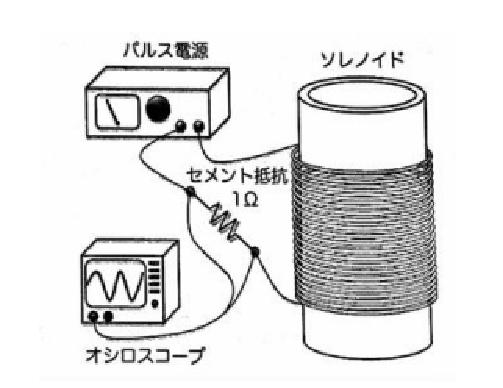
\includegraphics[scale=0.75]{figure1.pdf}
            \caption{実験装置}
        \end{center}
    \end{figure}
\end{enumerate}

\subsubsection{$L$の測定}
図1に示す実験配置において,パルス電流を流した際にセメント抵抗$(1\,\Omega)$の両端
にかかる電圧波形を記録する.ただし,パルス電源内には,$12\,\si{\mu F}$のコンデンサ
が入っており,$L$の計算を行う際には,セメント抵抗の抵抗値$(1\,\Omega)$は無視して
良いとする.さらに,電圧波形から周期$T$を測定することで,ソレノイドのインダクタンス
$L$の値を算出する.このときインダクタ$L$は,以下の式で算出される.
$$
L=\frac{r^2}{4\pi^2C}
$$


\subsubsection{$R$の決定}
実験課題1から算出したインダクタンス$L$の値を用いて,電流波形が臨界制動波形となる
際の$R$の値を計算し,実際にその抵抗$R$を回路に接続することで電流波形が
臨界制動波形となることを確認し,記録する.
このとき,抵抗値$R$は以下の式で算出される.
$$
R^2=\frac{4L}{C}
$$